\documentclass[11pt]{article}

\usepackage[a4paper, total={6in, 8in}]{geometry}
\usepackage{graphicx}
\usepackage{multicol,multirow}
\usepackage{enumitem}
\graphicspath{ {./Images/} }

\title{July2023 CSE300 Week10 Online Evaluation}
\author{2005020}
\date{\today}

\begin{document}
    \maketitle
    \tableofcontents

\newpage

\section{RISC Architecture}

\begin{figure}[!h]
    \centering
    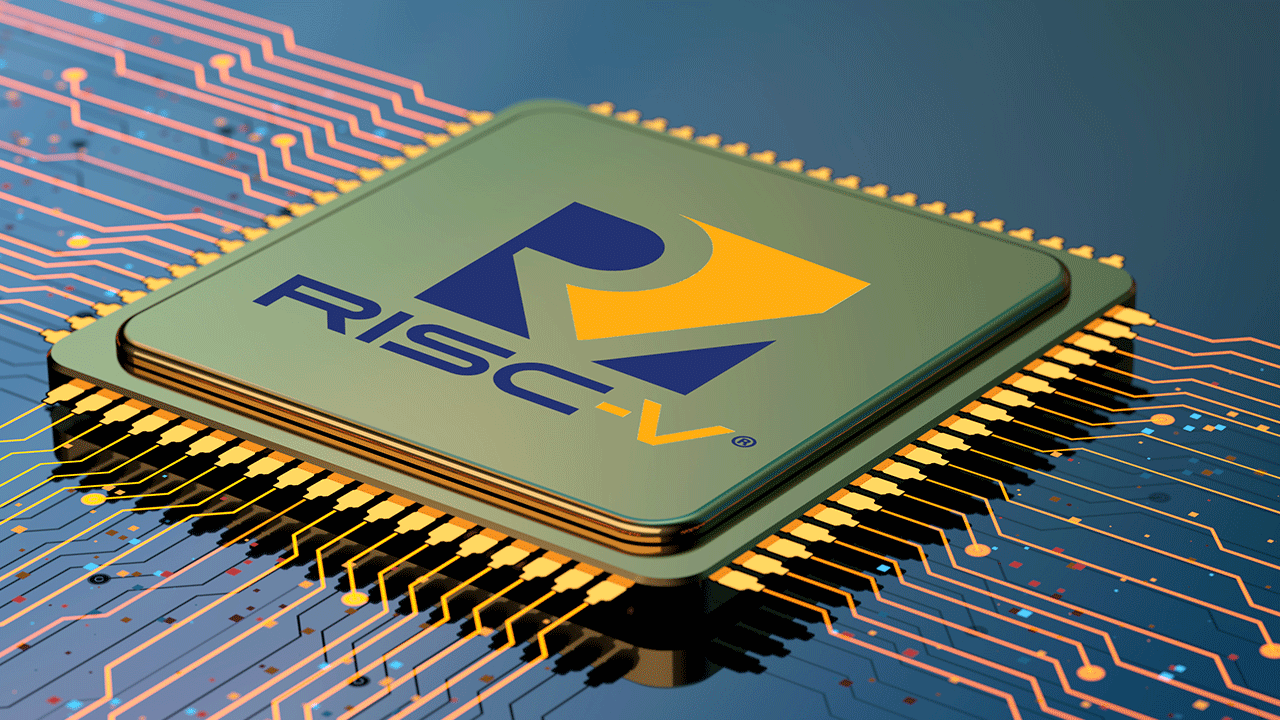
\includegraphics[width = 0.75\textwidth]{Images/risc.png}
    \caption{RISC Architecture}
    \label{fig:risc}
\end{figure}

\section{Tables in \LaTeX}

\begin{table}[!h]
    \centering
    \begin{tabular}{|c|l|c|c|}
        \hline
        \multirow{10}{*}{numeric literals} & \multirow{5}{*}{integers} & in decimal & \verb|8743| \\ \cline{3-4}
        & & \multirow{2}{*}{in octal} & \verb|0o7464| \\ \cline{4-4}
        & & & \verb|00103| \\ \cline{3-4}
        & & \multirow{2}{*}{in hexadecimal} & \verb|0x5A0FF| \\ \cline{4-4}
        & & & \verb|0xE0F2| \\ \cline{2-4}
        &  \multirow{5}{*}{fractionals} &  \multirow{5}{*}{in decimal} & \verb|140.58| \\ \cline{4-4}
        & & & \verb|8.04e7| \\ \cline{4-4}
        & & & \verb|0.34eE+12| \\ \cline{4-4}
        & & & \verb|5.4eE-12| \\ \cline{4-4}
        & & & \verb|47e22| \\ \hline
    \end{tabular}
    \caption{A table in \LaTeX}
    \label{tab:tab1}
\end{table}


Table 1 shows a table that contains cells spanning multiple columns and multiple rows.

\noindent \cite{2}
\newpage

\section{Writing Equations in Latex}

\begin{equation}
    L_{split} = \frac{1}{2}[\frac{G_{L}^{2}}{H_{L} + \lambda} + \frac{G_{R}^{2}}{H_{R} + \lambda} - 
    \frac{(G_{L} + G_{R})^{2}}{H_{L} + H_{R} + \lambda}] - \gamma
\end{equation}

Equation 1 has been displayed above \cite{1}

\section*{Untitled Section}

You need to display this section in your output PDF file. This section contains information
that may help you prepare the bibliography section. By the way, this section \textbf{will not
show up} in the table of contents.

\begin{enumerate}
    \item \textbf{Citation about the Greedy Forest Article}
    \begin{itemize}
        \item \textbf{Authors:} T. Zhang, R. Johnson
        \item \textbf{Title:} Learning nonlinear functions using regularized greedy forest
        \item \textbf{Year:} 2014
        \item \textbf{Journal} IEEE Transactions on Pattern Analysis and Machine Intelligence
    \end{itemize}
    \item \textbf{Citation about the Random Forest Article}
    \begin{itemize}
        \item \textbf{Author:} L. Breiman
        \item \textbf{Title:} Random Forests
        \item \textbf{Journal:} Machine Learning
        \item \textbf{Year:} 2001
    \end{itemize}
\end{enumerate}

\bibliographystyle{plain}
% \bibliographystyle{abbrv}
% \bibliographystyle{plain}

\bibliography{ref}
    
\end{document}